
\section{Process Orchestration + API \& Webinterface}
\label{sec:process_orchestration}



\subsection{Executer Classes: Training, Infilling, Validation}

The challenge for the foretold Web interface and API solution is to store different station data, independently and to dynamically control processes for each station. The root of the executer classes is to control the needed processes for Training, Infilling and Validation. Thus begins with passing the corresponding Station object to the executor class and for the process dedicated temporary folders are created, etc. The executors are designed as classes to allow for easy access to the different data of the process entity itself at all steps, from ERA5 download to plotting.

The Training Executer class is structured such that all needed inputs are directly passed on object creation, but the pipeline steps are initiated not from the class constructor but from an extra method called "execute" which allows for a similar "execute_with_sbatch" version which is useful when using the code stackon a super computer like levante.
The execution, first runs the download steps for the ERA5 data which is a combination of a few routines described in \autoref{sec:implementation}: Identifying the available timesteps, downloading the data, merging the .grib files, converting to NetCDF files and cropping in the space and time dimensions as described above. This is where the benefit of the work in the previous chapter comes into play, as all of that is controlled by just a few lines and even undisturbed of temp-folder management which is directly included in the routines from \autoref{sec:implementation}.
After completion of the preprocessing steps, when the necessary coherent training files are saved in the temp-folders of the executer object, it generates the training-args.txt which is used as the input parameters for the separate machine learning code stack. That file not only specifies how exactly the training should be executed and for how many iterations but also includes information about where there output, respectively the model files should be saved. As this is specified by one of the executer-objects properties, it is troublefree to handle the saving of the model wherever needed.

The Evaluation Executer used for the infilling routine is structured similarly to the Training Executer, but with the difference that the input parameters must include a model path, and that the download routines to obtain ERA5 data use the times where measurements are missing, instead of the times where measurements are available. The class has an execute function as well which runs the different steps after each other, but can be manipulated if certain steps such as the download of the ERA5 data should be run differently. The arguments .txt file for the CRAI module is generated similarly but of course with the parameters needed for evaluation.

The Validation Executer is structured similarly to the Evaluation Executer, but has the download routine of the Training Executor, to obtain the ERA5 data for the times when measurements are available. Also after the successful evaluation of the model, the plots for the comparison of the predictions with the actual measurements are generated and saved in the temp-folder of the executer object. The plots also are generated comfortably with the plotting routine from \autoref{sec:implementation}.

\subsection{Webinterface}

\begin{wrapfigure}[11]{r}{0.5\textwidth}
    \centering
    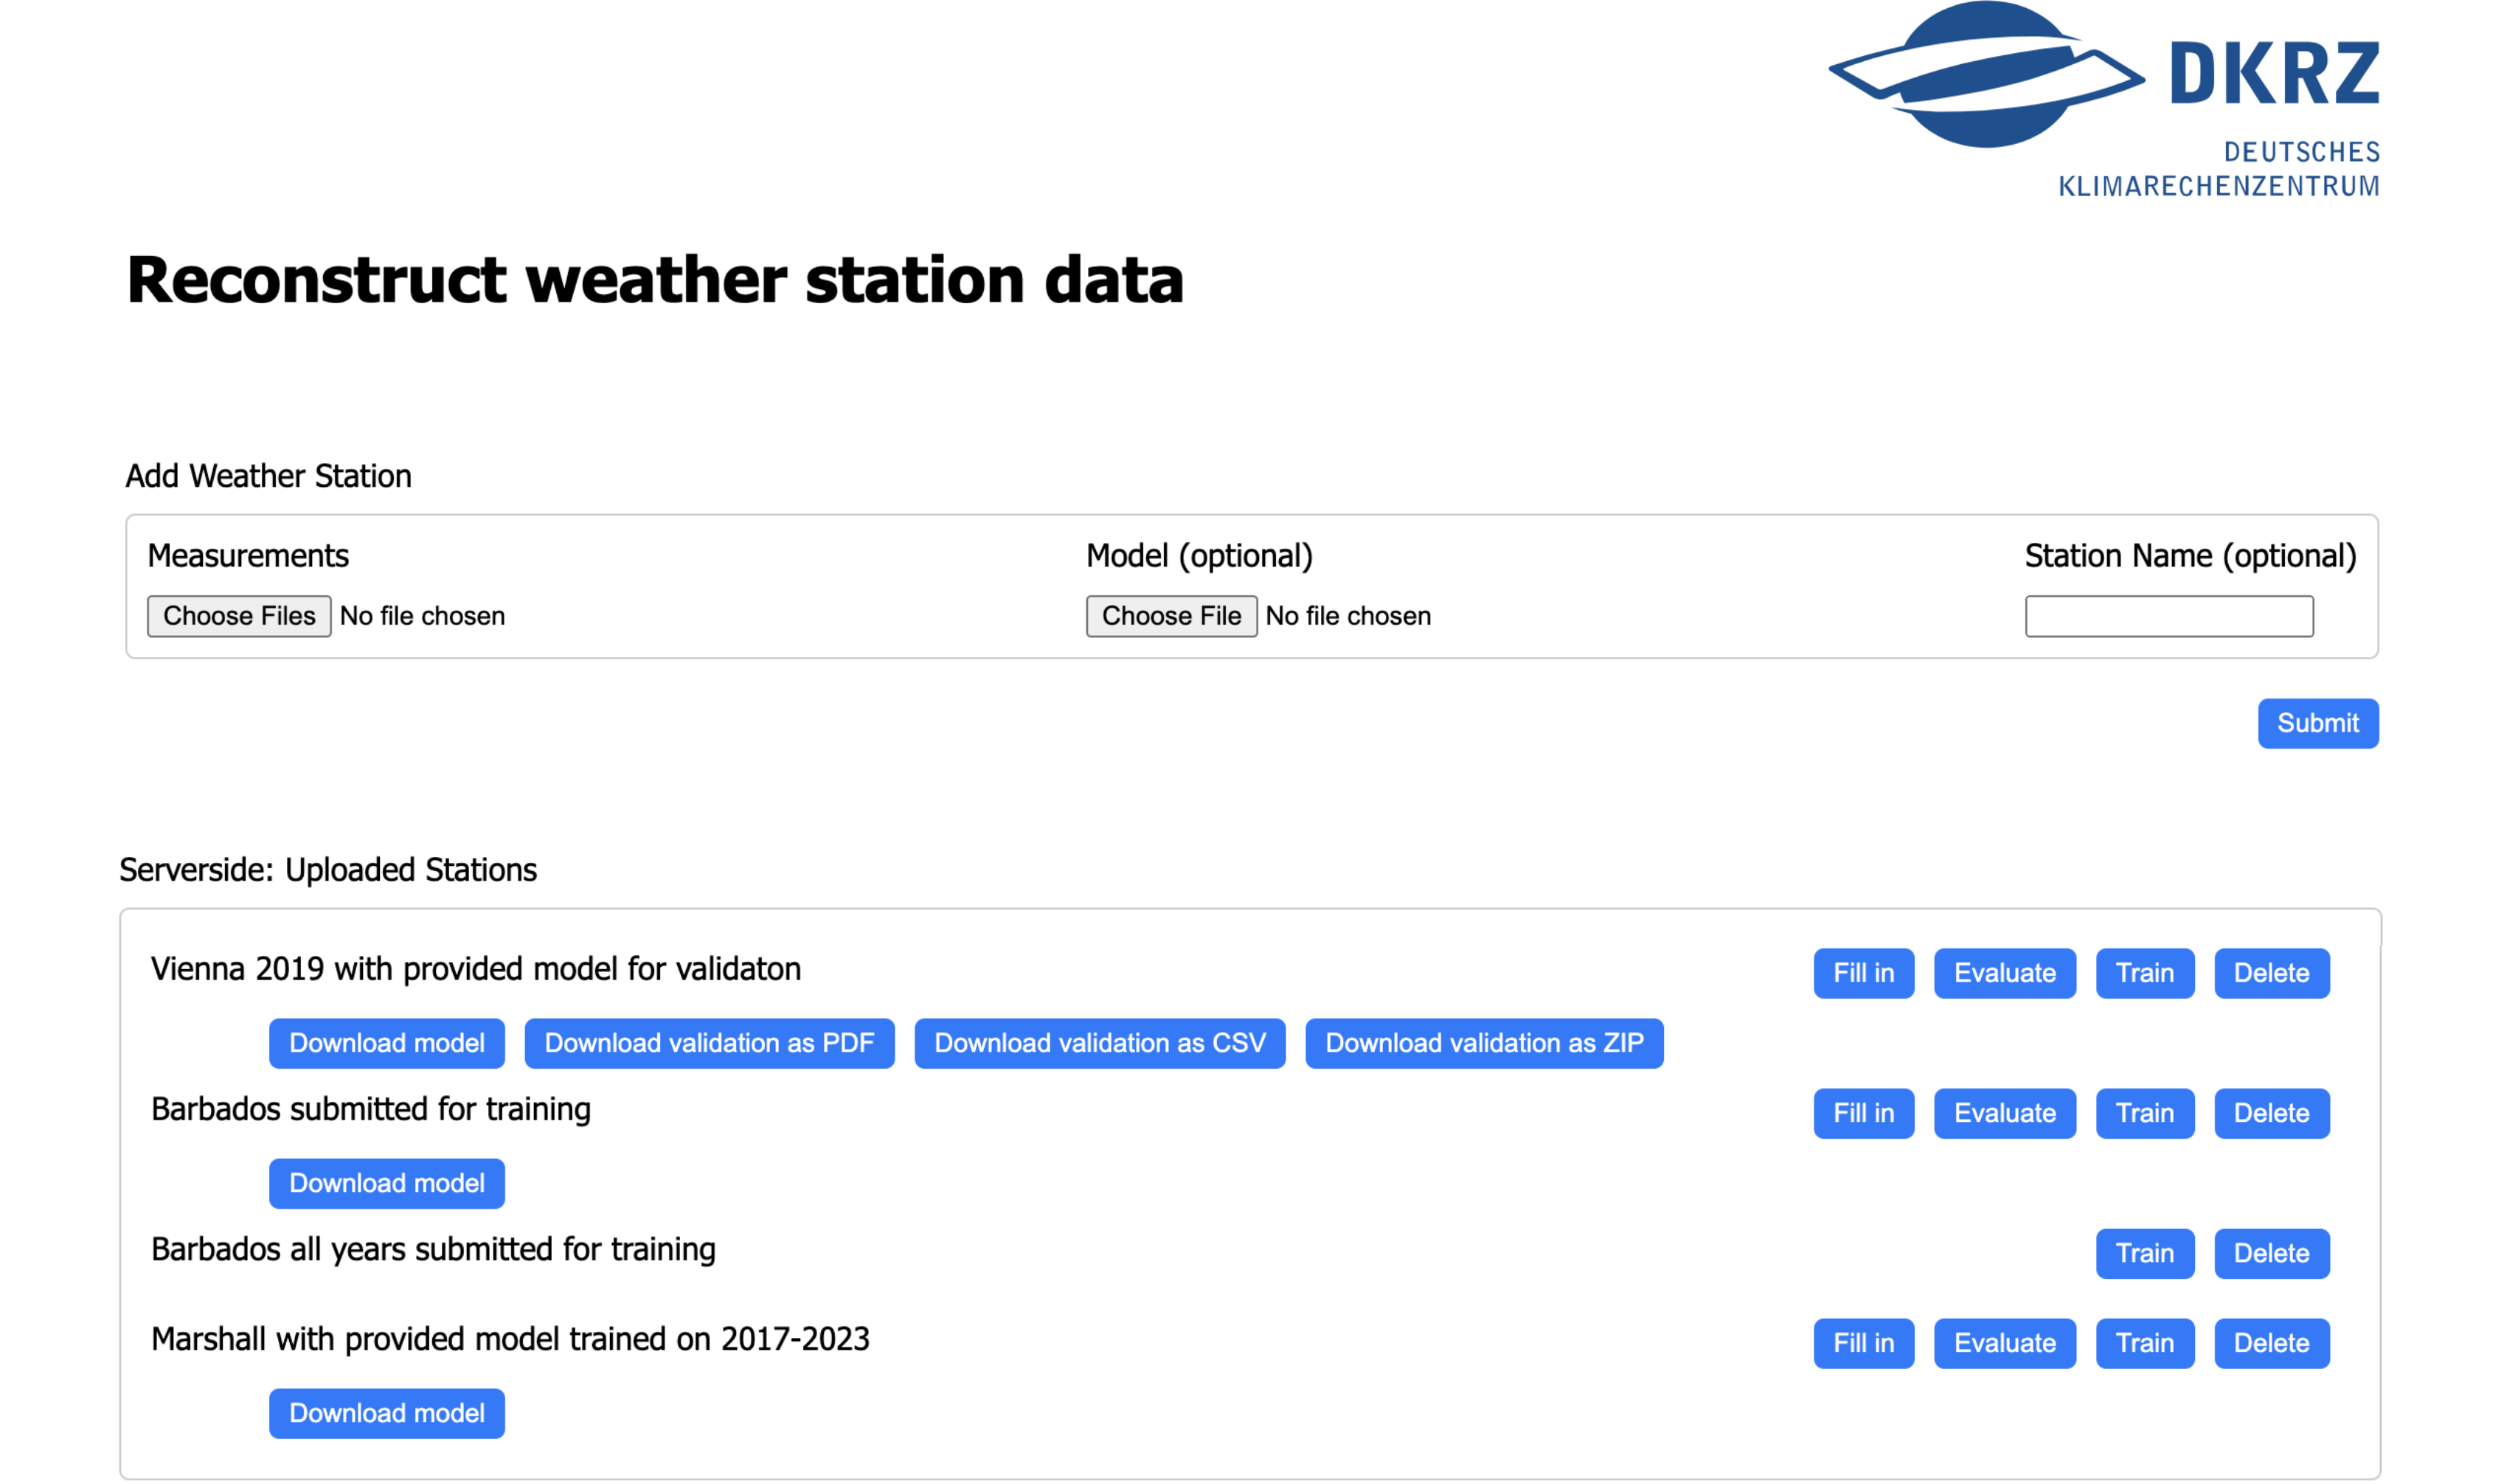
\includegraphics[width=0.5\textwidth]{resources/images/webinterface_screenshot.png}
    \caption{Screenshot of the webinterface}
    \label{fig:webinterface_screenshot}
\end{wrapfigure}

As written in the Introduction of this chapter \ref{sec:process_orchestration}, the benefit of establishing the abstraction layer with the executor classes is that with minimal additional effort, API Endpoints for initiation of processes to train/validate a model as well as endpoints to retrieve the results after the processes have finished. Additionally, it is possible to monitor the progress of the process through the API. The details on the API are described in \autoref{sec:api} This lays out a sufficient foundation for the implementation of a web interface, which is the main focus of this section.

The interface consists of two areas, one where the user is supposed to submit a "dataset", which in this context is meant as a collection of measurements from a weather station and the station's information such as location, and optionally a custom name and third a trained model for the station that can be provided optionally as well. If no model is provided the system can train a model and will attach it. 

The second area is a list of all datasets that the user has submitted. The API implementation allows for user identification through a unique token that is passed on to the server when the user submits a dataset, such that the user can then ask to see all datasets owned by them using that same token. The web interface automatically generates a token for the user and stores it then in the local storage of the browser, such that the user does not have to remember it.

As examples in \autoref{fig:webinterface_screenshot} show each dataset depending on its state has different options available. The deletion and train buttons all have in common, as no model is necessary to train a model. Datasets where a model has been provided still could be used to train a new model overwriting the old one. The "Evaluate" and "Fill in" buttons to evaluate the model over the timesteps where measurements are available, respectively to evaluate the model over the timesteps where measurements are missing.

Once a process such as training evaluation or infilling has been completed for a dataset the user can download the results anytime through the new buttons that appear in the dataset list. For example, it can be seen in \autoref{fig:webinterface_screenshot} that for the Vienna example, validation has been completed, and the user can now download a PDF with all the plots that compare the predictions with the actual measurements, or a CSV file with the same data, or a zip file that contains both and the images used in the PDF. The first Barbados example has a model attached that can be downloaded, meaning either it was provided or generated through training on the server itself. The second Barbados example has no model attached yet, meaning only the buttons "Train" and "Delete" are available, because no model was provided and no training has been done yet. 


\subsection{API Endpoints}
\label{sec:api}

% POST /data-submission
\subsubsection*{POST /data-submission}

Stores a new dataset on the server. Each dataset is associated with a unique ID, and a unique token representing the owner. The token of the owner is passed in the request body. The dataset ID is created by the server and returned in the response. The dataset ID is used to refer to the dataset in the following API calls.

% - GET /available-datasets/<user-token>
\subsubsection*{GET /available-datasets/<user-token>}

For a given user token, this endpoint returns a list of all datasets that the user has submitted. The user token is passed as a URL parameter. The response is a list of dictionaries, each containing information about the dataset, such as the dataset ID, the name, and the status of the dataset (e.g. if it is busy training a model and progress percentage).
% - GET /train/<data-submission-id>
\subsubsection*{GET /train/<data-submission-id>}

% - GET /validate-model/<dataset-id>
\subsubsection*{GET /validate-model/<dataset-id>}

% - GET /fill-in/<dataset-id>
\subsubsection*{GET /fill-in/<dataset-id>}

% - DELETE /delete-dataset/<dataset-id>
\subsubsection*{DELETE /delete-dataset/<dataset-id>}

% - GET /download-model/<dataset-id>
\subsubsection*{GET /download-model/<dataset-id>}

% - GET /download-validation-zip/<dataset-id> (just pdf and csv available too)
\subsubsection*{GET /download-validation-zip/<dataset-id>}

% - GET /download-infilling/<dataset-id>
\subsubsection*{GET /download-infilling/<dataset-id>}
